\documentclass[border=10pt]{standalone}

\usepackage{tikz}
\usepackage{tikzsymbols}
\usetikzlibrary{calc,patterns,shapes.geometric}

\def\centerarc[#1](#2)(#3:#4:#5){\draw[#1] ($(#2)+({#5*cos(#3)},{#5*sin(#3)})$) arc (#3:#4:#5);}

\begin{document}
	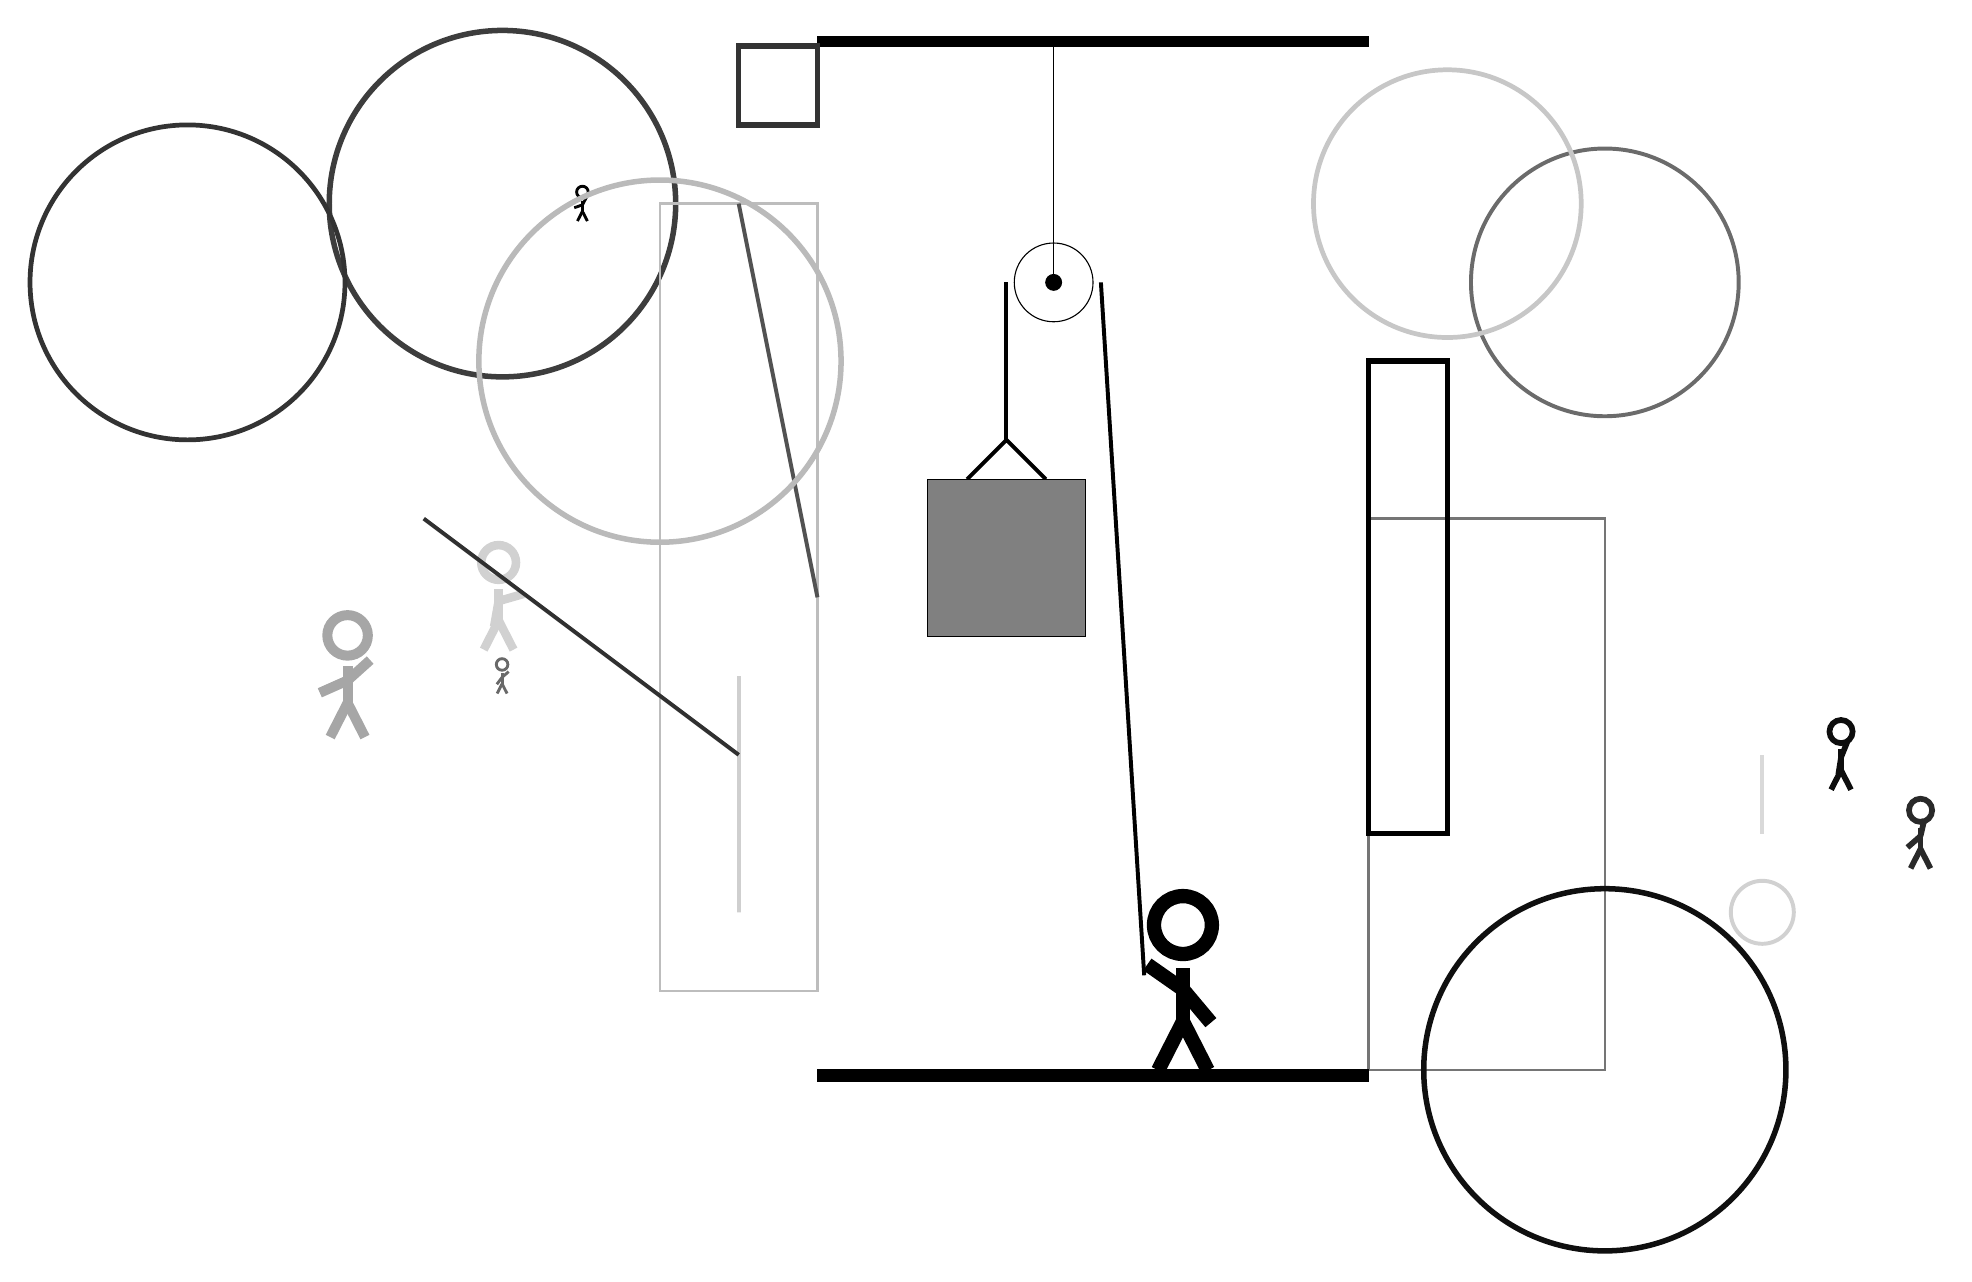
\begin{tikzpicture}
		%%%%% START %%%%%
		
		\draw[fill=black] (-2, 10) rectangle (5, 10.125);
		
		\draw (1, 7) circle (0.5);
		\draw[fill=black] (1, 7) circle (0.1);
		\draw (1, 10) -- (1, 7);
		
		\draw[line width=0.5mm] (-0.1, 4.5) -- (0.4, 5.0) -- (0.9, 4.5);
		\draw[fill=black!50] (-0.6, 4.5) rectangle (1.4, 2.5);
		
		\draw[line width=0.5mm] (0.4, 7) -- (0.4, 5.0);
		\centerarc[line width=0.5mm](1, 7)(0:180:0.6);
		\draw[line width=0.5mm](1.6, 7) -- (2.15, -1.8);
		
		\draw[line width=0.7mm, color=black!80] (-2, 9) rectangle (-3, 10);
		
		\node[line width=0.3mm, color=black!18] at (-6, 3) {\Strichmaxerl[6][80][16]};
		\node[line width=0.4mm, color=black!59] at (-6, 2) {\Strichmaxerl[2][53][41]};
		\draw[line width=0.3mm, color=black!54] (5, 4) rectangle (8, -3);
		\draw [line width=0.7mm, color=black!76](-6, 8) circle (2.2);
		\draw[line width=0.7mm, color=black!37] (5, 4) rectangle (5, 5);
		\draw[line width=0.3mm, color=black!26] (-2, 8) rectangle (-4, -2);
		\draw [line width=0.5mm, color=black!18](10, -1) circle (0.4);
		\draw [line width=0.7mm, color=black!94](8, -3) circle (2.3);
		\node[line width=0.6mm, color=black!84] at (12, 0) {\Strichmaxerl[4][41][77]};
		\draw [line width=0.5mm, color=black!58](8, 7) circle (1.7);
		\draw[line width=0.5mm, color=black!19] (-3, -1) rectangle (-3, 2);
		\node[line width=0.7mm, color=black!95] at (11, 1) {\Strichmaxerl[4][81][68]};
		
		\draw [line width=0.6mm, color=black!80](-10, 7) circle (2.0);
		\draw[line width=0.5mm, color=black!15](10, 0) -- (10, 1);
		\draw[line width=0.5mm, color=black!81](-7, 4) -- (-3, 1);
		
		\node[line width=0.6mm, color=black!99] at (-5, 8) {\Strichmaxerl[2][19][62]};
		\draw[line width=0.5mm, color=black!68](-3, 8) -- (-2, 3);
		\draw [line width=0.7mm, color=black!27](-4, 6) circle (2.3);
		\draw [line width=0.6mm, color=black!22](6, 8) circle (1.7);
		\node[line width=0.5mm, color=black!35] at (-8, 2) {\Strichmaxerl[7][24][42]};
		
		\draw[line width=0.7mm, color=black!100] (6, 6) rectangle (5, 0);
		
		
		\node at (2.6, -1.9) {\Strichmaxerl[10][-35][-50]};
		
		\draw[fill=black] (-2, -3) rectangle (5, -3.15);
		
		%%%%% END %%%%%
	\end{tikzpicture}
\end{document}